\documentclass[12pt,]{article}
\usepackage{lmodern}
\usepackage{amssymb,amsmath}
\usepackage{ifxetex,ifluatex}
\usepackage{fixltx2e} % provides \textsubscript
\ifnum 0\ifxetex 1\fi\ifluatex 1\fi=0 % if pdftex
  \usepackage[T1]{fontenc}
  \usepackage[utf8]{inputenc}
\else % if luatex or xelatex
  \ifxetex
    \usepackage{mathspec}
  \else
    \usepackage{fontspec}
  \fi
  \defaultfontfeatures{Ligatures=TeX,Scale=MatchLowercase}
    \setmainfont[]{Times New Roman}
\fi
% use upquote if available, for straight quotes in verbatim environments
\IfFileExists{upquote.sty}{\usepackage{upquote}}{}
% use microtype if available
\IfFileExists{microtype.sty}{%
\usepackage{microtype}
\UseMicrotypeSet[protrusion]{basicmath} % disable protrusion for tt fonts
}{}
\usepackage[margin=2.54cm]{geometry}
\usepackage{hyperref}
\hypersetup{unicode=true,
            pdftitle={Policy Analysis of California Clean Air Act on the Reduction of PM2.5 in Bay Area Counties},
            pdfauthor={Wanchen Xiong},
            pdfborder={0 0 0},
            breaklinks=true}
\urlstyle{same}  % don't use monospace font for urls
\usepackage{color}
\usepackage{fancyvrb}
\newcommand{\VerbBar}{|}
\newcommand{\VERB}{\Verb[commandchars=\\\{\}]}
\DefineVerbatimEnvironment{Highlighting}{Verbatim}{commandchars=\\\{\}}
% Add ',fontsize=\small' for more characters per line
\usepackage{framed}
\definecolor{shadecolor}{RGB}{248,248,248}
\newenvironment{Shaded}{\begin{snugshade}}{\end{snugshade}}
\newcommand{\KeywordTok}[1]{\textcolor[rgb]{0.13,0.29,0.53}{\textbf{#1}}}
\newcommand{\DataTypeTok}[1]{\textcolor[rgb]{0.13,0.29,0.53}{#1}}
\newcommand{\DecValTok}[1]{\textcolor[rgb]{0.00,0.00,0.81}{#1}}
\newcommand{\BaseNTok}[1]{\textcolor[rgb]{0.00,0.00,0.81}{#1}}
\newcommand{\FloatTok}[1]{\textcolor[rgb]{0.00,0.00,0.81}{#1}}
\newcommand{\ConstantTok}[1]{\textcolor[rgb]{0.00,0.00,0.00}{#1}}
\newcommand{\CharTok}[1]{\textcolor[rgb]{0.31,0.60,0.02}{#1}}
\newcommand{\SpecialCharTok}[1]{\textcolor[rgb]{0.00,0.00,0.00}{#1}}
\newcommand{\StringTok}[1]{\textcolor[rgb]{0.31,0.60,0.02}{#1}}
\newcommand{\VerbatimStringTok}[1]{\textcolor[rgb]{0.31,0.60,0.02}{#1}}
\newcommand{\SpecialStringTok}[1]{\textcolor[rgb]{0.31,0.60,0.02}{#1}}
\newcommand{\ImportTok}[1]{#1}
\newcommand{\CommentTok}[1]{\textcolor[rgb]{0.56,0.35,0.01}{\textit{#1}}}
\newcommand{\DocumentationTok}[1]{\textcolor[rgb]{0.56,0.35,0.01}{\textbf{\textit{#1}}}}
\newcommand{\AnnotationTok}[1]{\textcolor[rgb]{0.56,0.35,0.01}{\textbf{\textit{#1}}}}
\newcommand{\CommentVarTok}[1]{\textcolor[rgb]{0.56,0.35,0.01}{\textbf{\textit{#1}}}}
\newcommand{\OtherTok}[1]{\textcolor[rgb]{0.56,0.35,0.01}{#1}}
\newcommand{\FunctionTok}[1]{\textcolor[rgb]{0.00,0.00,0.00}{#1}}
\newcommand{\VariableTok}[1]{\textcolor[rgb]{0.00,0.00,0.00}{#1}}
\newcommand{\ControlFlowTok}[1]{\textcolor[rgb]{0.13,0.29,0.53}{\textbf{#1}}}
\newcommand{\OperatorTok}[1]{\textcolor[rgb]{0.81,0.36,0.00}{\textbf{#1}}}
\newcommand{\BuiltInTok}[1]{#1}
\newcommand{\ExtensionTok}[1]{#1}
\newcommand{\PreprocessorTok}[1]{\textcolor[rgb]{0.56,0.35,0.01}{\textit{#1}}}
\newcommand{\AttributeTok}[1]{\textcolor[rgb]{0.77,0.63,0.00}{#1}}
\newcommand{\RegionMarkerTok}[1]{#1}
\newcommand{\InformationTok}[1]{\textcolor[rgb]{0.56,0.35,0.01}{\textbf{\textit{#1}}}}
\newcommand{\WarningTok}[1]{\textcolor[rgb]{0.56,0.35,0.01}{\textbf{\textit{#1}}}}
\newcommand{\AlertTok}[1]{\textcolor[rgb]{0.94,0.16,0.16}{#1}}
\newcommand{\ErrorTok}[1]{\textcolor[rgb]{0.64,0.00,0.00}{\textbf{#1}}}
\newcommand{\NormalTok}[1]{#1}
\usepackage{longtable,booktabs}
\usepackage{graphicx,grffile}
\makeatletter
\def\maxwidth{\ifdim\Gin@nat@width>\linewidth\linewidth\else\Gin@nat@width\fi}
\def\maxheight{\ifdim\Gin@nat@height>\textheight\textheight\else\Gin@nat@height\fi}
\makeatother
% Scale images if necessary, so that they will not overflow the page
% margins by default, and it is still possible to overwrite the defaults
% using explicit options in \includegraphics[width, height, ...]{}
\setkeys{Gin}{width=\maxwidth,height=\maxheight,keepaspectratio}
\IfFileExists{parskip.sty}{%
\usepackage{parskip}
}{% else
\setlength{\parindent}{0pt}
\setlength{\parskip}{6pt plus 2pt minus 1pt}
}
\setlength{\emergencystretch}{3em}  % prevent overfull lines
\providecommand{\tightlist}{%
  \setlength{\itemsep}{0pt}\setlength{\parskip}{0pt}}
\setcounter{secnumdepth}{5}
% Redefines (sub)paragraphs to behave more like sections
\ifx\paragraph\undefined\else
\let\oldparagraph\paragraph
\renewcommand{\paragraph}[1]{\oldparagraph{#1}\mbox{}}
\fi
\ifx\subparagraph\undefined\else
\let\oldsubparagraph\subparagraph
\renewcommand{\subparagraph}[1]{\oldsubparagraph{#1}\mbox{}}
\fi

%%% Use protect on footnotes to avoid problems with footnotes in titles
\let\rmarkdownfootnote\footnote%
\def\footnote{\protect\rmarkdownfootnote}

%%% Change title format to be more compact
\usepackage{titling}

% Create subtitle command for use in maketitle
\newcommand{\subtitle}[1]{
  \posttitle{
    \begin{center}\large#1\end{center}
    }
}

\setlength{\droptitle}{-2em}

  \title{Policy Analysis of California Clean Air Act on the Reduction of PM2.5 in
Bay Area Counties}
    \pretitle{\vspace{\droptitle}\centering\huge}
  \posttitle{\par}
  \subtitle{Web address for GitHub repository}
  \author{Wanchen Xiong}
    \preauthor{\centering\large\emph}
  \postauthor{\par}
    \date{}
    \predate{}\postdate{}
  

\begin{document}
\maketitle
\begin{abstract}
Experimental overview. This section should be no longer than 250 words.
\end{abstract}

\newpage

\tableofcontents  \newpage

\section{Research Question and
Rationale}\label{research-question-and-rationale}

Air pollution is an important aspects of environmental quality
management. There have been numerous studies showing the adverse health
effects of air pollutants, such as ozone, particulate matter, nitrogen
oxide, lead and so on. In the United States, there have been progress in
establishing legislations to control these air pollutants since the
Clean Air Act of 1970, which established the federal framework to reduce
air pollutants from stationary and mobile sources. This project chose
PM2.5, ambient particulate matters with a diameter of 2.5 micrometers
that have been studied extensively to be proved to have devastating
effects on human lungs and cardiovascular systems. And the area of
interest is bay area in northern California, as California has been
progressive in implementing state air quality management programs and
the bay area is both the political, industrial, and urban hub of the
state. The state of California established a new annual standard for
daily maximum PM2.5 of 12 ug/m3 in June, 2002, and this standard became
effective in 2003. Therefore, this environmental data analysis project
is investigating whether this policy intervention led to significant
reduction of ambient PM2.5 in bay area over the years since it's
effective. Meanwhile, California has frequent natural disaster such as
wildfires annually, so this project will explore whether air monitoring
captures such temporal variability of air quality and provide meaningful
data support for management.

This analysis is developed into 4 research questions:

\begin{itemize}
\item
  \begin{enumerate}
  \def\labelenumi{\arabic{enumi}.}
  \tightlist
  \item
    Overall reduction across the bay area: Is there a signficant
    reduction in PM2.5 from 1999 to 2016 in the bay area(9 counties)? Is
    the ambient PM2.5 concentration after the policy significantly less
    comparing to that before the policy was implemented?
  \end{enumerate}
\item
  \begin{enumerate}
  \def\labelenumi{\arabic{enumi}.}
  \setcounter{enumi}{1}
  \tightlist
  \item
    Is each county having significant reduction in its ambient PM2.5?
    How does this comparison look like geographically?
  \end{enumerate}
\item
  \begin{enumerate}
  \def\labelenumi{\arabic{enumi}.}
  \setcounter{enumi}{2}
  \tightlist
  \item
    Looking at one bay area county, Santa Clara County, is there a point
    of change since the policy change? A time series analysis was
    performed to look at when the data reflects a change in the trend of
    ambient PM2.5.
  \end{enumerate}
\item
  \begin{enumerate}
  \def\labelenumi{\arabic{enumi}.}
  \setcounter{enumi}{3}
  \tightlist
  \item
    Is the air monitoring data capturing temporary events such as
    wildfires? Solano County had three wildfires over the year 2018 and
    was explored to investigate the effectiveness of the air monitoring
    data.
  \end{enumerate}
\end{itemize}

\newpage

\section{Dataset Information}\label{dataset-information}

The air monitoring data for PM2.5 were collected from
\href{https://www.epa.gov/outdoor-air-quality-data/download-daily-data}{here}.
PM2.5 data for California are available from 1999 to 2018. These data
were archived by year. Each file included the daily maximum PM2.5
concentration and the date recorded were continuously from January 1 to
Decomber 31 for each year(though some days were missing in some years).
All the available PM2.5 data were downloaded as individual csv files and
will be combined and wrangled for the analysis of this projet.

The spatial data included the California county boundaries were from
California governmental open data
\href{https://data.ca.gov/dataset/ca-geographic-boundaries/resource/091ff50d-bb24-4537-a974-2ce89c6e8663}{here}
and will be used for spatial analysis in this project.

\begin{longtable}[]{@{}ll@{}}
\toprule
\begin{minipage}[b]{0.35\columnwidth}\raggedright\strut
Data Name\strut
\end{minipage} & \begin{minipage}[b]{0.56\columnwidth}\raggedright\strut
Information\strut
\end{minipage}\tabularnewline
\midrule
\endhead
\begin{minipage}[t]{0.35\columnwidth}\raggedright\strut
EPA Air Quality PM2.5\strut
\end{minipage} & \begin{minipage}[t]{0.56\columnwidth}\raggedright\strut
The dataset contains data from air quality monitoring of PM2.5 in
California from 1999 to 2018. All the data are in csv formats and named
as pm\_year\_ca.\strut
\end{minipage}\tabularnewline
\begin{minipage}[t]{0.35\columnwidth}\raggedright\strut
California County Boundary\strut
\end{minipage} & \begin{minipage}[t]{0.56\columnwidth}\raggedright\strut
The dataset contains the shapefile for all the county boundaries in
California.\strut
\end{minipage}\tabularnewline
\bottomrule
\end{longtable}

\newpage

\section{Exploratory Data Analysis and
Wrangling}\label{exploratory-data-analysis-and-wrangling}

After pulling in all the PM2.5 monitoring data from 1999 to 2018, a data
wrangling is performed to only include 9 bay area counties, and make
sure date is in the right format and recognized by R. Save the processed
data to the folder.

\begin{Shaded}
\begin{Highlighting}[]
\CommentTok{# wrangle this new dataframe to only include 9 bay area counties}
\CommentTok{# Make sure date is in the right format and recognized by R. Save the processed data to the folder.}

\NormalTok{bay_pm_99_}\DecValTok{18}\NormalTok{ <-}
\StringTok{  }\NormalTok{ca_pm_99_}\DecValTok{18} \OperatorTok
\StringTok{  }\KeywordTok{filter}\NormalTok{(COUNTY }\OperatorTok{==}\StringTok{ "Alameda"} \OperatorTok{|}
\StringTok{                   }\NormalTok{COUNTY }\OperatorTok{==}\StringTok{ "Contra Costa"} \OperatorTok{|}
\StringTok{                   }\NormalTok{COUNTY }\OperatorTok{==}\StringTok{ "Marin"} \OperatorTok{|}
\StringTok{                   }\NormalTok{COUNTY }\OperatorTok{==}\StringTok{ "Napa"} \OperatorTok{|}
\StringTok{                   }\NormalTok{COUNTY }\OperatorTok{==}\StringTok{ "San Francisco"} \OperatorTok{|}
\StringTok{                   }\NormalTok{COUNTY }\OperatorTok{==}\StringTok{ "San Mateo"} \OperatorTok{|}
\StringTok{                   }\NormalTok{COUNTY }\OperatorTok{==}\StringTok{ "Santa Clara"} \OperatorTok{|}
\StringTok{                   }\NormalTok{COUNTY }\OperatorTok{==}\StringTok{ "Solano"} \OperatorTok{|}
\StringTok{                   }\NormalTok{COUNTY }\OperatorTok{==}\StringTok{ "Sonoma"}\NormalTok{) }\OperatorTok
\StringTok{  }\KeywordTok{select}\NormalTok{(Date, Site.ID, Daily.Mean.PM2.}\FloatTok{5.}\NormalTok{Concentration, UNITS, DAILY_AQI_VALUE, }
\NormalTok{         COUNTY, SITE_LATITUDE, SITE_LONGITUDE)}
\NormalTok{bay_pm_99_}\DecValTok{18} \OperatorTok{$}\NormalTok{Date <-}\StringTok{ }\KeywordTok{as.Date}\NormalTok{(bay_pm_99_}\DecValTok{18} \OperatorTok{$}\NormalTok{Date, }\DataTypeTok{format =} \StringTok{"%m/%d/%Y"}\NormalTok{)}
\NormalTok{bay_pm_99_}\DecValTok{18}\NormalTok{  <-}\StringTok{ }\KeywordTok{mutate}\NormalTok{(bay_pm_99_}\DecValTok{18}\NormalTok{ , }
                        \DataTypeTok{month =} \KeywordTok{month}\NormalTok{(}\KeywordTok{as.Date}\NormalTok{(bay_pm_99_}\DecValTok{18}\OperatorTok{$}\NormalTok{Date, }\StringTok{"%Y-%m-%d"}\NormalTok{)))}
\NormalTok{bay_pm_99_}\DecValTok{18}\NormalTok{  <-}\StringTok{ }\KeywordTok{mutate}\NormalTok{(bay_pm_99_}\DecValTok{18}\NormalTok{ , }
                        \DataTypeTok{year =} \KeywordTok{year}\NormalTok{(}\KeywordTok{as.Date}\NormalTok{(bay_pm_99_}\DecValTok{18} \OperatorTok{$}\NormalTok{Date, }\StringTok{"%Y-%m-%d"}\NormalTok{)))}
\NormalTok{bay_pm_99_}\DecValTok{18} \OperatorTok{$}\NormalTok{year <-}\StringTok{ }\KeywordTok{as.factor}\NormalTok{(bay_pm_99_}\DecValTok{18} \OperatorTok{$}\NormalTok{year)}

\CommentTok{# Save the processed data into the "processed" folder.}
\KeywordTok{write.csv}\NormalTok{(bay_pm_99_}\DecValTok{18}\NormalTok{, }\DataTypeTok{file =} \StringTok{"./Processed/bay_pm25_99to18.csv"}\NormalTok{)}
\end{Highlighting}
\end{Shaded}

\begin{Shaded}
\begin{Highlighting}[]
\CommentTok{# Display the data's structure, dimension, columns and have a look at first/last several columns}
\KeywordTok{str}\NormalTok{(bay_pm_99_}\DecValTok{18}\NormalTok{)}

\KeywordTok{dim}\NormalTok{(bay_pm_99_}\DecValTok{18}\NormalTok{)}

\KeywordTok{colnames}\NormalTok{(bay_pm_99_}\DecValTok{18}\NormalTok{)}

\KeywordTok{head}\NormalTok{(bay_pm_99_}\DecValTok{18}\NormalTok{)}

\KeywordTok{tail}\NormalTok{(bay_pm_99_}\DecValTok{18}\NormalTok{)}
\end{Highlighting}
\end{Shaded}

\newpage

After data is wrangled, a clean dataframe that includes the necessary
information for the purpose of this analysis is produced. However, in
order to proceed to data analysis and create meaningful synthesis of the
data, initial data exploration is necessary.

Therefore, several plots were produced to look at the patterns of the
concentration of PM2.5 by county and by year to identify potential
interesting factors that are worth exploring in addition to the research
goals.

First, figure 1 is produced to look at each of the 9 bay area counties
and their respective PM2.5 concentration level over 1999-2018.

\begin{figure}
\centering
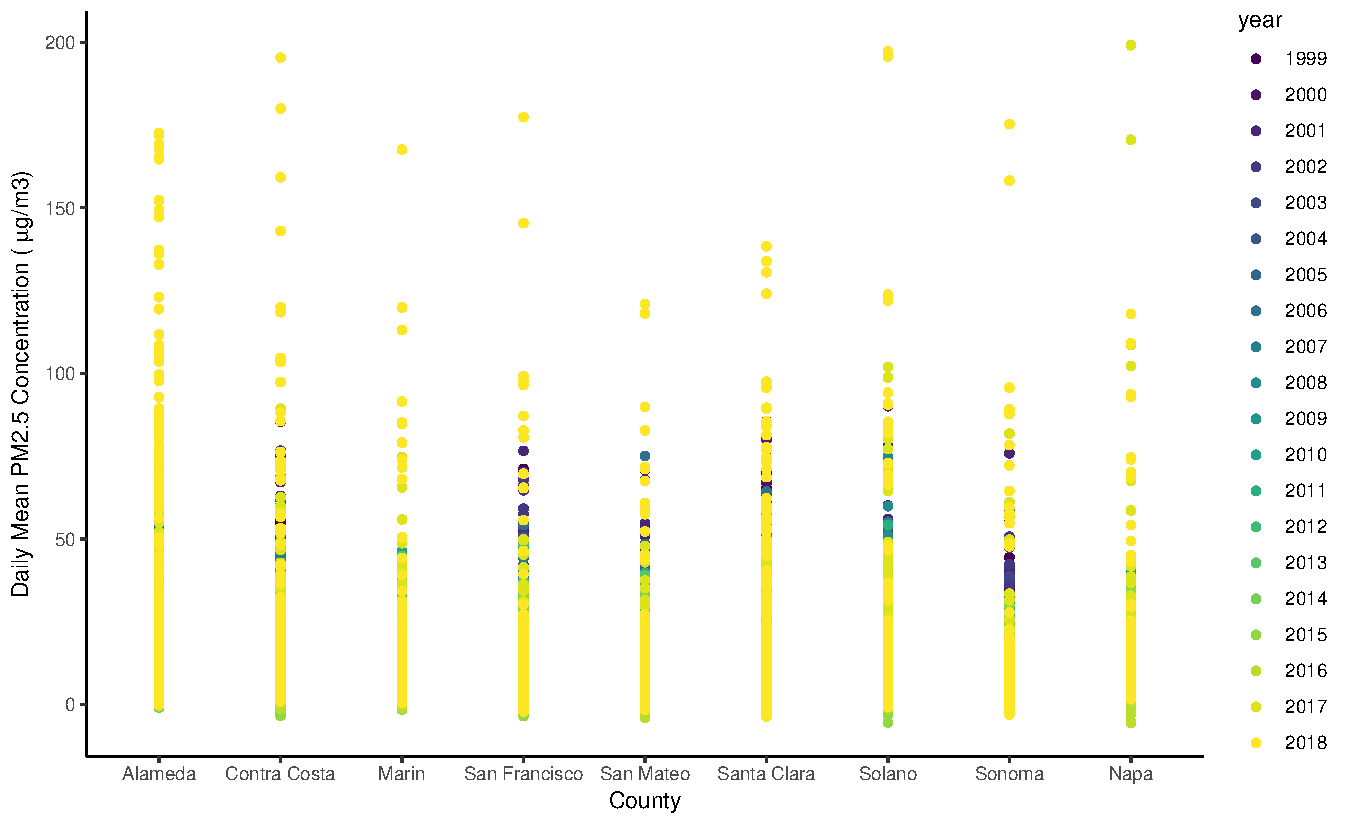
\includegraphics{pm25_files/figure-latex/explore1-1.pdf}
\caption{Data Exploration: 9 Bay Area Counties and PM2.5}
\end{figure}

Then, figure 2 is generated to identify if there is seasonal effects
that influence ambient PM2.5.

\begin{figure}
\centering
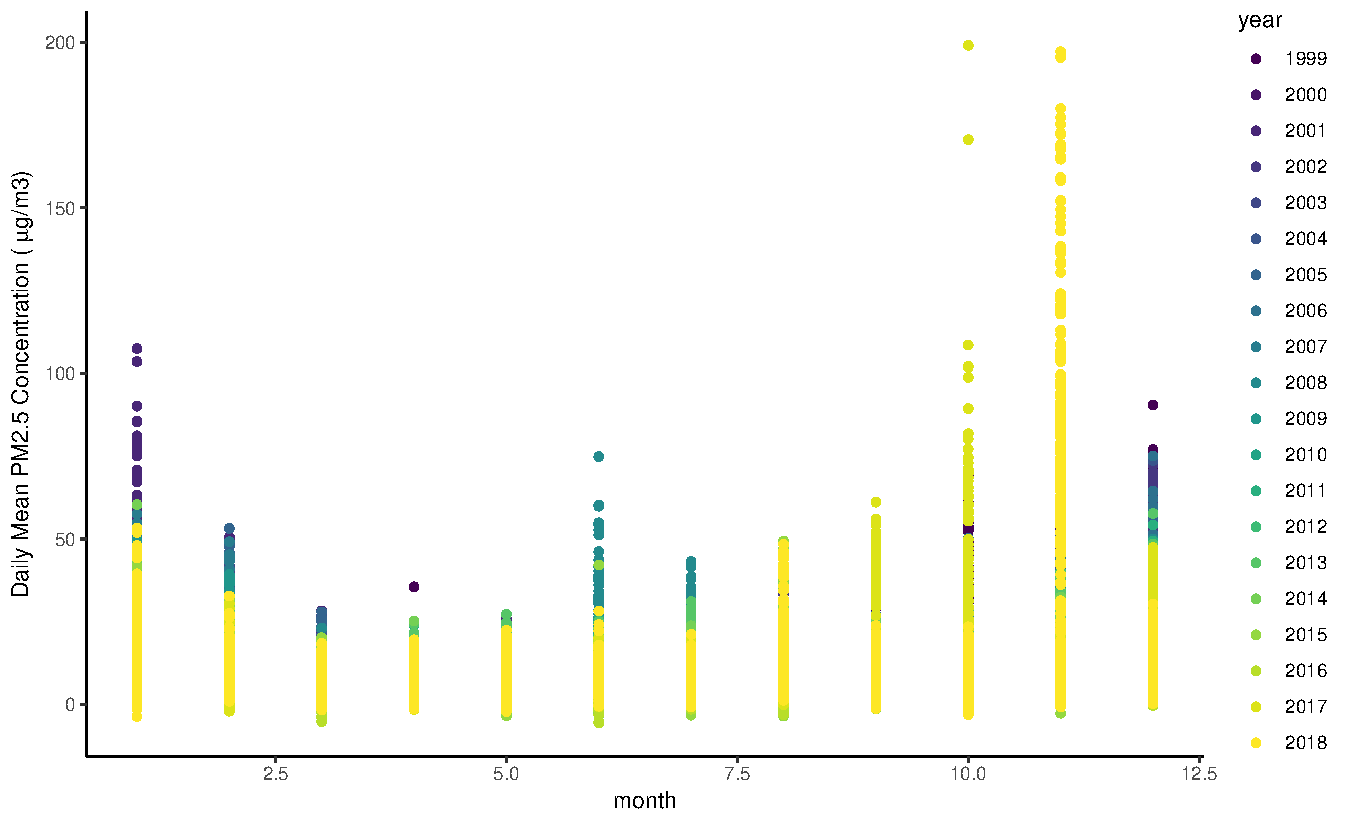
\includegraphics{pm25_files/figure-latex/explore2-1.pdf}
\caption{Data Exploration: Is There Seasonal Variability of PM2.5?}
\end{figure}

After looking at the first and second exploration plot, it looks like
2017 and 2018 have some extreme data out of the normal range. Therefore,
for the purpose of this project, data from 2017 and 2018 will be
excluded for the most part except when California wild fire events were
considered for the last research question.

Figure 3 is generated to explore which county has the best and worst air
pollution based on PM2.5 concentration.

\begin{figure}
\centering
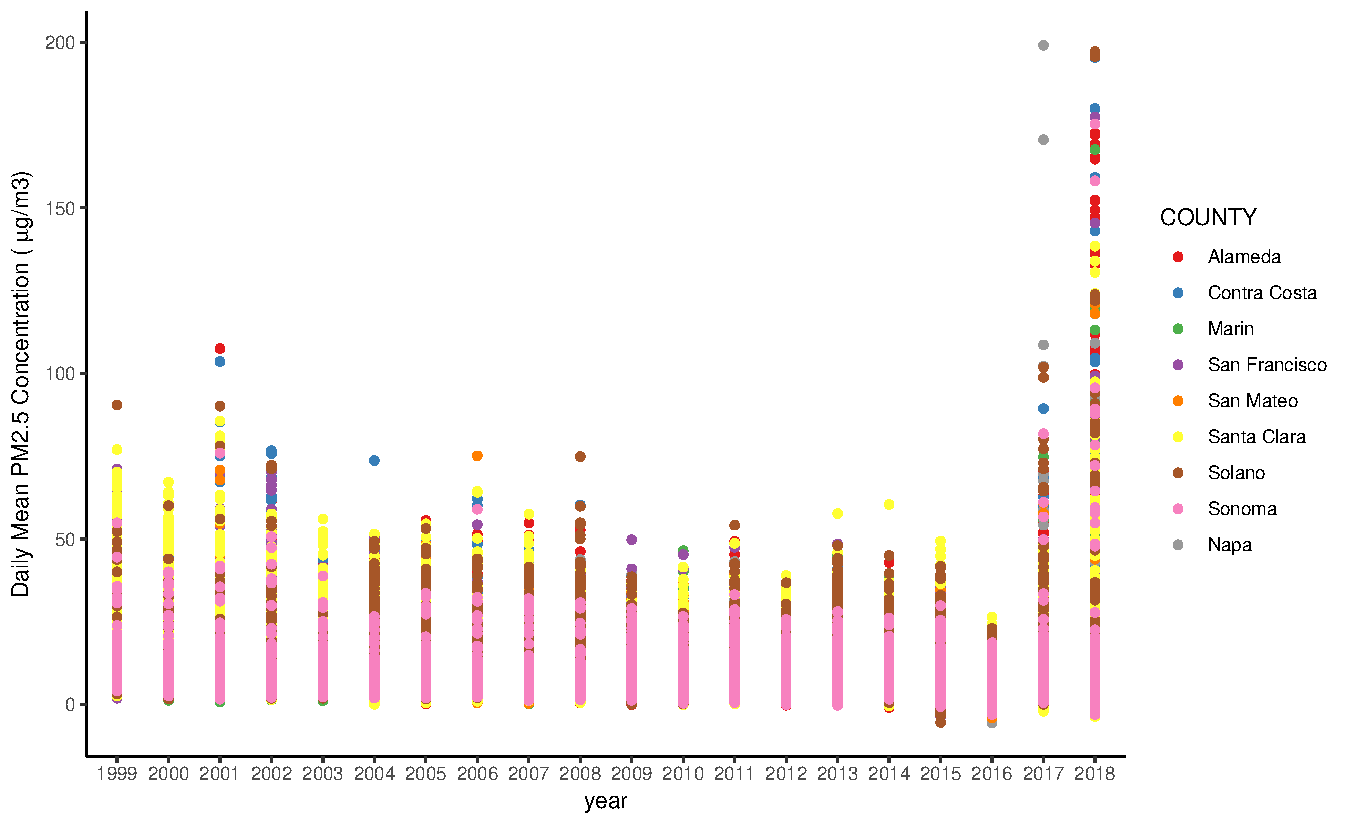
\includegraphics{pm25_files/figure-latex/explore3-1.pdf}
\caption{Data Exploration: Comparison among Counties}
\end{figure}

\newpage

\section{Analysis}\label{analysis}

\subsection{Research Question 1: Is PM2.5 Reducing in Bay Area
?}\label{research-question-1-is-pm2.5-reducing-in-bay-area}

Since California implemented the PM2.5 standard in 2003. The data before
2003 will be referred as ``before the state regulation'', whereas data
after 2003 will be referred as ``after the state regulation''.

Perform a t test to see whether there is:

\begin{enumerate}
\def\labelenumi{\arabic{enumi})}
\item
  a significant change in PM2.5 concentration across the bay area before
  and after the state started regulating PM2.5;
\item
  a decrease in the PM2.5 concentration since the state regulation was
  effective.
\end{enumerate}

The results of the T-test shows that there is a significant difference
in PM2.5 concentration for all 9 counties as a whole between before the
regulation and after the regulation; the test shows that there is a
reduction of 4.35 micrograms/cubic meter for the bay area since the
regulation (p \textless{} 0.0001, mean difference = 4.35 with 95 CI).

Figure 4 is a graphic result of the T-test.

\begin{figure}
\centering
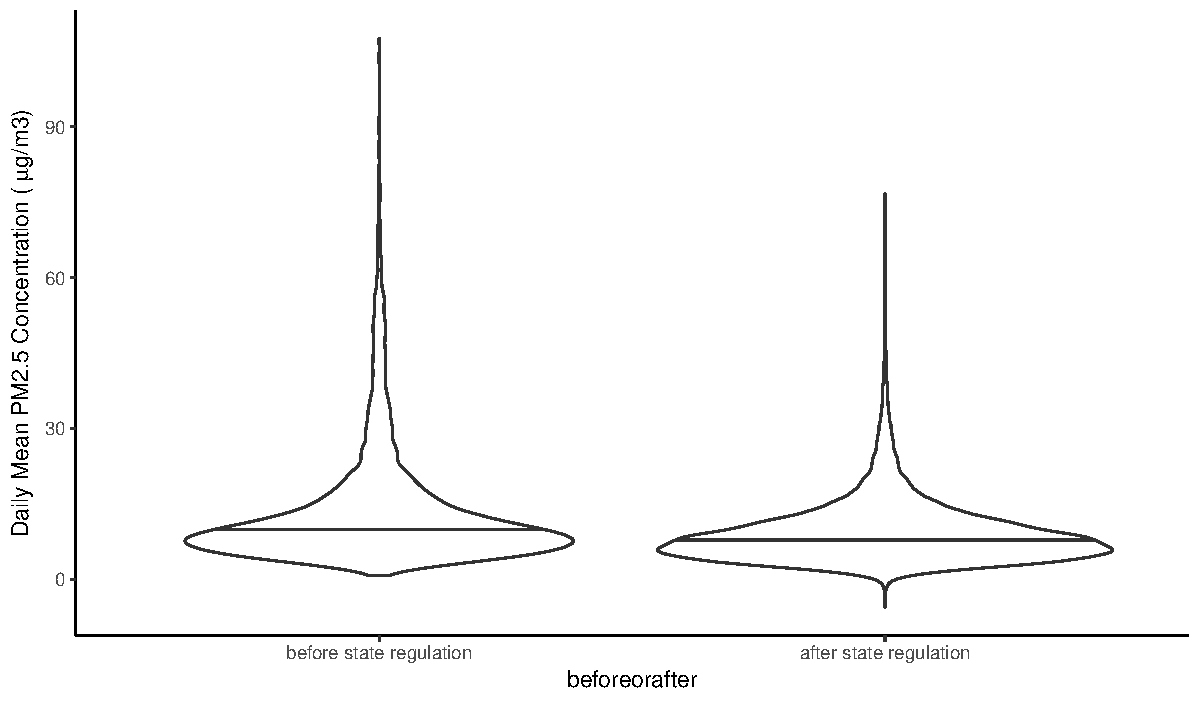
\includegraphics{pm25_files/figure-latex/unnamed-chunk-3-1.pdf}
\caption{Difference in Mean PM2.5 before- and after-regulation}
\end{figure}

Figure 5 displays the an overall change in PM2.5 concentration before
the regulation and after the regulation.

\begin{figure}
\centering
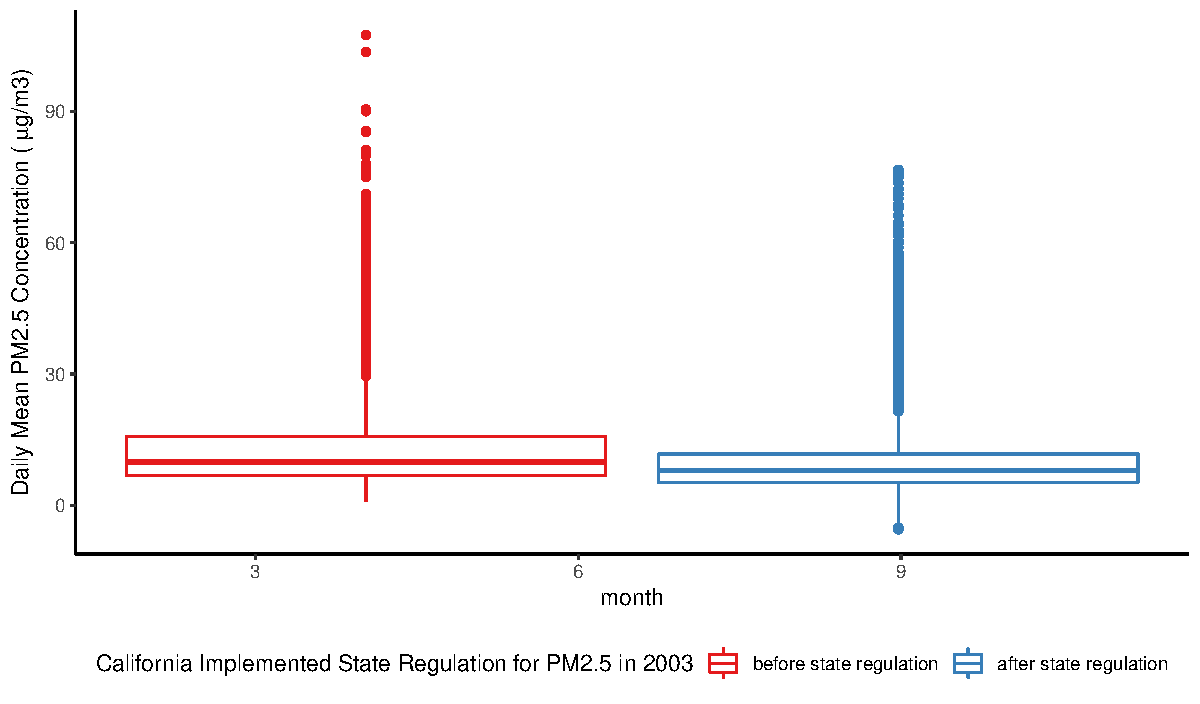
\includegraphics{pm25_files/figure-latex/unnamed-chunk-4-1.pdf}
\caption{Mean PM2.5 Across 9 Bay Area Counties}
\end{figure}

\newpage

\subsection{Research Question 2: How Does Each County Experience Change
in PM2.5
?}\label{research-question-2-how-does-each-county-experience-change-in-pm2.5}

After running the statistical test on all of the bay area counties as a
whole, a signficant reduction in PM2.5 is observed. To further explore
this trend, a T-test is performed to see whether every county in bay
area is reducing its PM2.5. Since Napa county does not have data before
the regulation, it is excluded from this analysis. The following code is
a T-test performed on Alameda County.

\begin{Shaded}
\begin{Highlighting}[]
\CommentTok{# First, wrangle the data to divide Alameda PM2.5 data into before- and after-regulation.}
\NormalTok{Alameda.be <-}\StringTok{ }\NormalTok{before_reg }\OperatorTok
\StringTok{  }\KeywordTok{filter}\NormalTok{(COUNTY }\OperatorTok{==}\StringTok{ "Alameda"}\NormalTok{)}
\NormalTok{Alameda.af <-}\StringTok{ }\NormalTok{after_reg }\OperatorTok
\StringTok{  }\KeywordTok{filter}\NormalTok{(COUNTY }\OperatorTok{==}\StringTok{ "Alameda"}\NormalTok{)}

\CommentTok{# Run a T-test Alameda County to see if it has reduced in PM2.5 since 2002.    }
\KeywordTok{t.test}\NormalTok{(Alameda.be}\OperatorTok{$}\NormalTok{Daily.Mean.PM2.}\FloatTok{5.}\NormalTok{Concentration, }
\NormalTok{       Alameda.af}\OperatorTok{$}\NormalTok{Daily.Mean.PM2.}\FloatTok{5.}\NormalTok{Concentration, }\DataTypeTok{alternative =} \StringTok{"greater"}\NormalTok{)}
\end{Highlighting}
\end{Shaded}

Run the same test for each of the 8 counties. A result is summarized in
this table:

\begin{longtable}[]{@{}ll@{}}
\toprule
County Name & Results\tabularnewline
\midrule
\endhead
Alameda & Significant reduction, mean differnce = -3.89
(p\textless{}0.0001)\tabularnewline
Contra Costa & Significant reduction, mean differnce = -4.30
(p\textless{}0.0001)\tabularnewline
Marin & No significant change, mean difference = +1.38 (p =
1)\tabularnewline
San Francisco & Singificant reduction, mean difference = -4.16
(p\textless{}0.0001)\tabularnewline
San Mateo & Significant reduction, mean difference = -2.49
(p\textless{}0.0001)\tabularnewline
Santa Clara & significant reduction, mean difference = -5.59
(p\textless{}0.0001)\tabularnewline
Solano & Significant reduction, mean difference = -3.60
(p\textless{}0.0001)\tabularnewline
Sonoma & Significant reduction, mean difference = -3.37
(p\textless{}0.0001)\tabularnewline
\bottomrule
\end{longtable}

As seen in figure 6, every county except Marin county shows a signficant
reduction in PM2.5 concentration since the regulation. Even though Marin
County seems to show a non-significant increase in PM2.5, Marin County
is already at the lower end of PM2.5 level to begin with, comparing to
the rest of the counties.

\begin{figure}
\centering
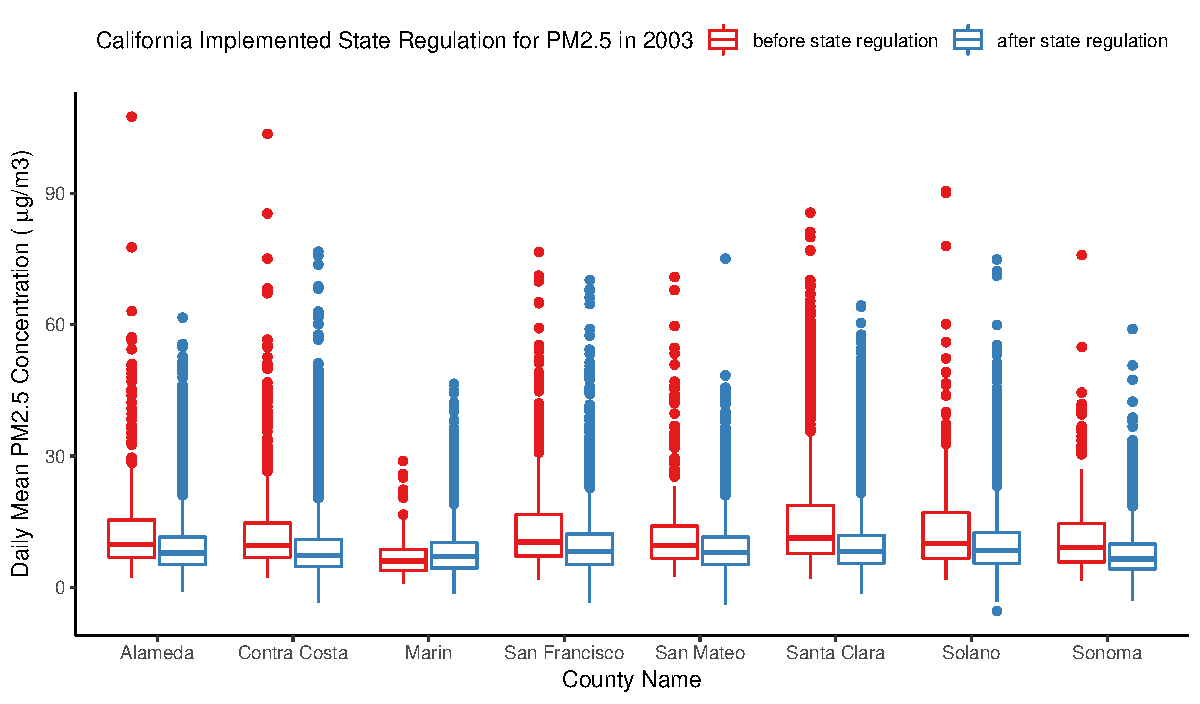
\includegraphics{pm25_files/figure-latex/unnamed-chunk-7-1.pdf}
\caption{PM2.5 Comparison Before and After Regulation for 8 Bay Area
Counties}
\end{figure}

\newpage

\subsection{The Spatial Display of the Results of the
Regulation}\label{the-spatial-display-of-the-results-of-the-regulation}

Figure 7 and figure 8 shows the level of air pollution regarding PM2.5
concentration in a spatial display. The color is calibrated at the
regulation standard, PM2.5 = 12 micrograms/cubic meter. The more orange
the county is, the higher the PM2.5 concentration is. The more blue the
county is, the lower the PM2.5 concentration is. The majority of PM2.5
high level seems to concentrate in the eastern part of the Bay Area,
where it is mostly inland and urban environment.

\begin{figure}
\centering
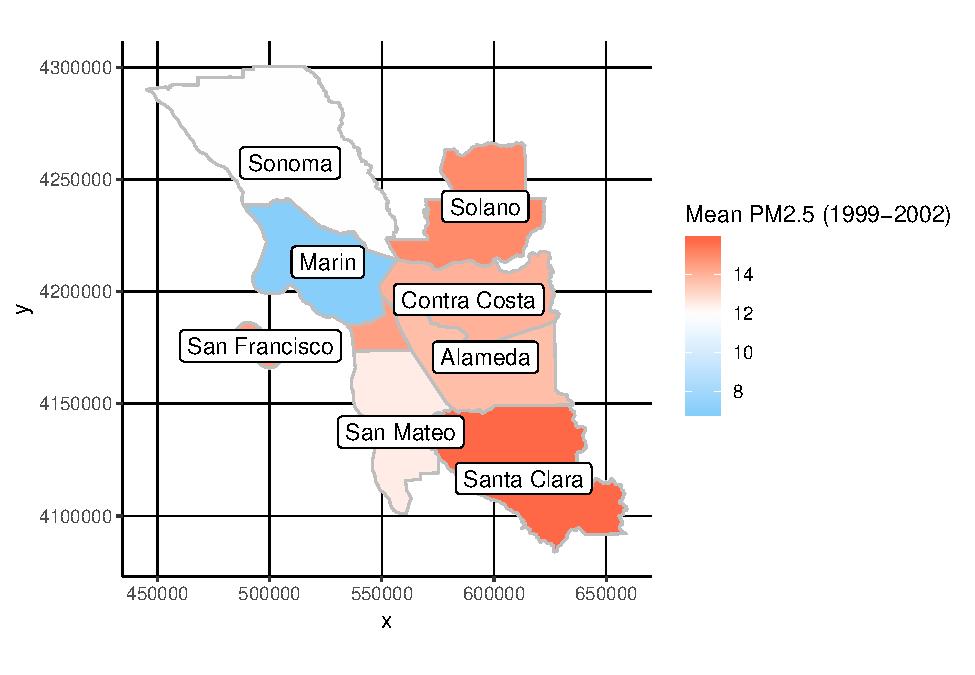
\includegraphics{pm25_files/figure-latex/unnamed-chunk-9-1.pdf}
\caption{Mean PM2.5 in Each Bay Area County Before 2003}
\end{figure}

\begin{figure}
\centering
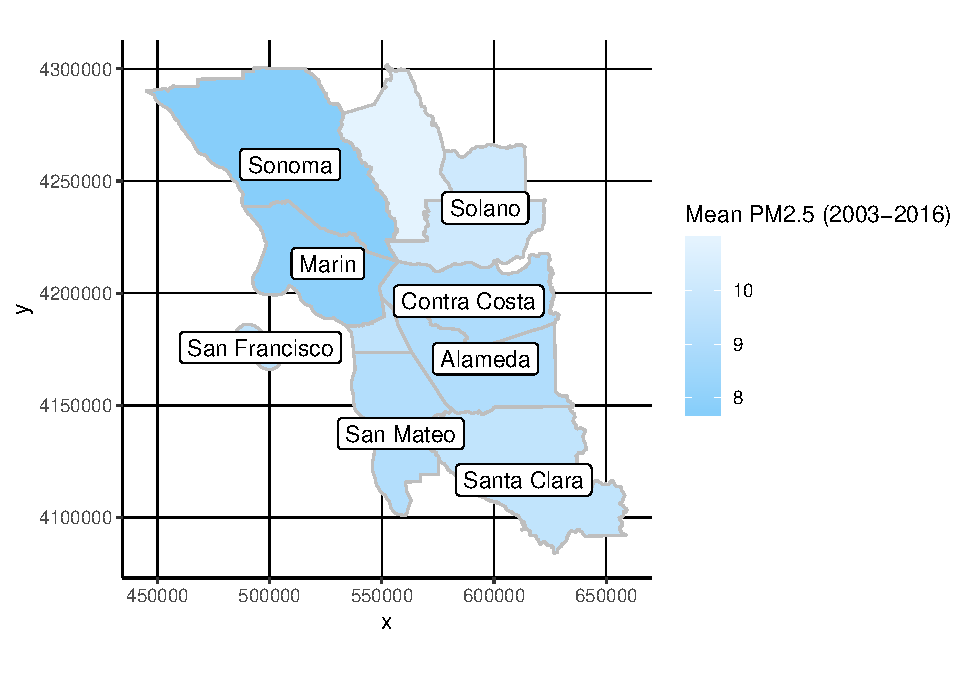
\includegraphics{pm25_files/figure-latex/unnamed-chunk-10-1.pdf}
\caption{Mean PM2.5 in Each Bay Area County After 2003}
\end{figure}

\newpage

\subsection{Research Question 3: Is There a Point of Change in the Data
to Reflect the Effectiveness of the Regulation? A Close Look at Santa
Clara
County.}\label{research-question-3-is-there-a-point-of-change-in-the-data-to-reflect-the-effectiveness-of-the-regulation-a-close-look-at-santa-clara-county.}

First, ingle out Santa Clara County and wrangle the data to just include
data for Santa Clara County and from year 1999 to 2016.

Perform a time series analysis using Mann-Kendall trend test to see
whether there is a trend in the PM2.5 concentration over time.

\begin{Shaded}
\begin{Highlighting}[]
\CommentTok{# Perform the time series analysis on Santa Clara County}
\KeywordTok{mk.test}\NormalTok{(sc_pm_99_}\DecValTok{16}\OperatorTok{$}\NormalTok{Daily.Mean.PM2.}\FloatTok{5.}\NormalTok{Concentration)}
\end{Highlighting}
\end{Shaded}

The result shows that there is a significant negative trend from 1999 to
2016 (z = -27.29, p \textless{} 0.0001).

\begin{Shaded}
\begin{Highlighting}[]
\CommentTok{# Perform a pettitt test to detect where is the changing point in the data}
\KeywordTok{pettitt.test}\NormalTok{(sc_pm_99_}\DecValTok{16}\OperatorTok{$}\NormalTok{Daily.Mean.PM2.}\FloatTok{5.}\NormalTok{Concentration)}
\end{Highlighting}
\end{Shaded}

Pettitt's test shows that there is a point of change occurred at
location 5463(P\textless{}0.0001), which refers to Februry 4, 2009. This
seems a reasonable time for the regulation to take effecst. However,
more investigation of the data is needed before any conclusion can be
made. Perform another Mann-Kendall trend test and pettitt test to see
whether there is a trend in between the starting date to Februry 4,
2009.

\begin{Shaded}
\begin{Highlighting}[]
\CommentTok{# Perform another pettitt test to see whether there is a trend.}
\KeywordTok{mk.test}\NormalTok{(sc_pm_99_}\DecValTok{16}\OperatorTok{$}\NormalTok{Daily.Mean.PM2.}\FloatTok{5.}\NormalTok{Concentration[}\DecValTok{1}\OperatorTok{:}\DecValTok{5463}\NormalTok{])}
\KeywordTok{pettitt.test}\NormalTok{(sc_pm_99_}\DecValTok{16}\OperatorTok{$}\NormalTok{Daily.Mean.PM2.}\FloatTok{5.}\NormalTok{Concentration[}\DecValTok{1}\OperatorTok{:}\DecValTok{5463}\NormalTok{])}
\end{Highlighting}
\end{Shaded}

The Mann-Kendall trend test shows that there is a significant negative
trend leading up to Februry 4, 2009(z = -10.33, P\textless{}0.0001). And
the result of pettitt test shows that the point of change occurs at
position 2108, which refers to Feb 1, 2003. This looks like a reasonable
estimation of the time that it takes for the policy to take effects. To
check that this is the first turning point, perform another round of
Mann-Kendall trend test and pettitt test to validate this conclusion.

\begin{Shaded}
\begin{Highlighting}[]
\CommentTok{# Perform another Mann-Kendall trend test and pettitt test}
\KeywordTok{mk.test}\NormalTok{(sc_pm_99_}\DecValTok{16}\OperatorTok{$}\NormalTok{Daily.Mean.PM2.}\FloatTok{5.}\NormalTok{Concentration[}\DecValTok{1}\OperatorTok{:}\DecValTok{2108}\NormalTok{])}
\KeywordTok{pettitt.test}\NormalTok{(sc_pm_99_}\DecValTok{16}\OperatorTok{$}\NormalTok{Daily.Mean.PM2.}\FloatTok{5.}\NormalTok{Concentration[}\DecValTok{1}\OperatorTok{:}\DecValTok{2108}\NormalTok{])}
\end{Highlighting}
\end{Shaded}

The result shows that the trend of ambient PM2.5 is a negative one as it
approaches Feb 1, 2003. The pettitt test again to see if there is any
significant point of change before Feb 1, 2003 and after 2003. The
result shows that at location 350, which equals to Jan 12, 2000, is a
possible point of change; however, this date falls out of range of our
interest because we are only interested in the time after the regulation
was implemented. Therefore, since the state regulation was effective in
2003, the first significant change of point occurs on Feb 1, 2003.

Figure 9 presents the change in the ambient PM2.5 concentration,
separated by months, since 1999 to 2016.

\begin{figure}
\centering
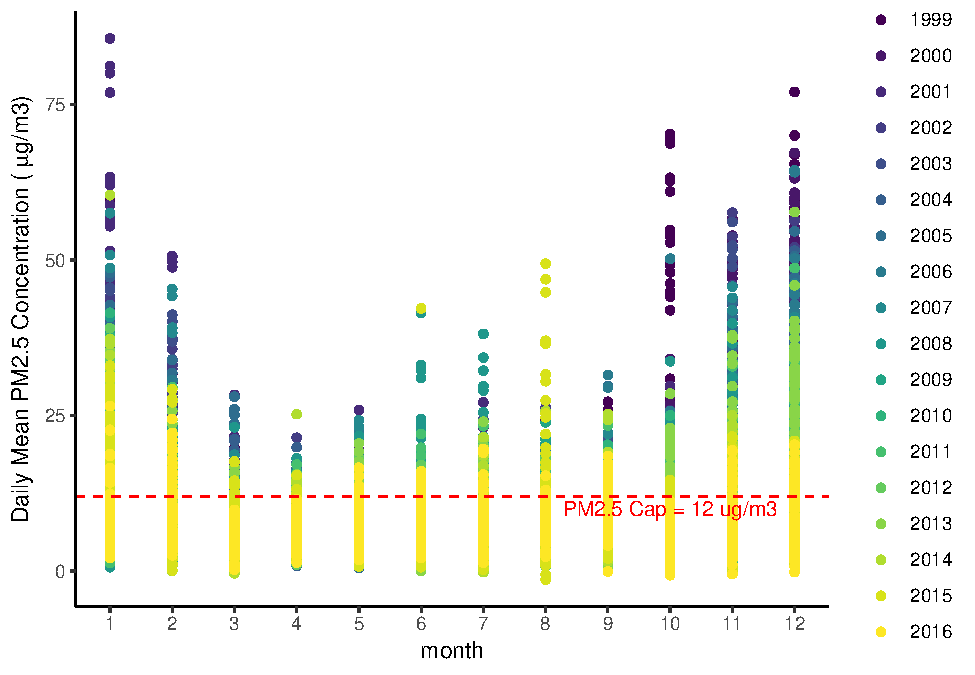
\includegraphics{pm25_files/figure-latex/unnamed-chunk-16-1.pdf}
\caption{PM2.5 Concentration Trend from 1999 to 2016 in Santa Clara
County}
\end{figure}

\newpage

\subsection{Research Question 4: Does EPA Air Quality Monitoring Data
Capture Air Pollution Disturbance like Wildfire? A Close Look at Solano
County in
2018.}\label{research-question-4-does-epa-air-quality-monitoring-data-capture-air-pollution-disturbance-like-wildfire-a-close-look-at-solano-county-in-2018.}

EPA air quality data are used by policymakers, researchers, and
environmental management professionals frequently. Therefore, it is
important that these data accurately reflect what's happening in the
environment. PM2.5 is a large component of the pollutants emitted from
fire. This section explores the PM2.5 data for Solano County in 2018 to
see if it correctly captures the wildfires events happened in this
county on August 10, Oct 7, and November 8, 2018.

\begin{Shaded}
\begin{Highlighting}[]
\CommentTok{# Perform an anova test to see if there is a significant difference between }
\CommentTok{# August, October, and November comparing to reference month, January, which}
\CommentTok{# no fire event happened.}
\NormalTok{PM2.}\FloatTok{5.}\NormalTok{anova <-}\StringTok{ }\KeywordTok{lm}\NormalTok{(solano_pm_}\DecValTok{18}\OperatorTok{$}\NormalTok{Daily.Mean.PM2.}\FloatTok{5.}\NormalTok{Concentration }
                  \OperatorTok{~}\StringTok{ }\NormalTok{solano_pm_}\DecValTok{18}\OperatorTok{$}\NormalTok{month)}
\KeywordTok{summary}\NormalTok{(PM2.}\FloatTok{5.}\NormalTok{anova)}
\end{Highlighting}
\end{Shaded}

The result shows that November's mean PM2.5 concentration is
significantly different from the reference month (P \textless{} 0.0001).
Therefore, the difference between month that has wildfire and the month
that does not is only reflective of November, as shown in Figure 10.

However, this test does not conclude that the data are not accurate.
There are days that are missing, especially during the second fire
event, which half of month's data were missing. Therefore, this might
lead to the result that the expected worse air pollution is not
reflected in the data.

\begin{figure}
\centering
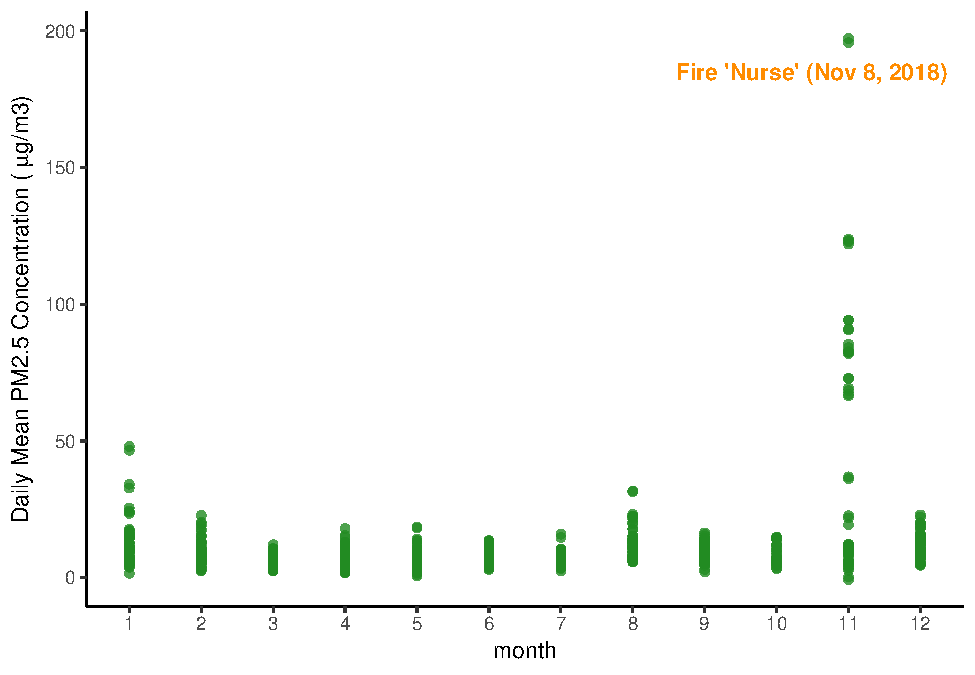
\includegraphics{pm25_files/figure-latex/unnamed-chunk-19-1.pdf}
\caption{Overview of PM2.5 Concentration in 2018, Solano County}
\end{figure}

\newpage

\section{Summary and Conclusions}\label{summary-and-conclusions}

Policy interventions in air quality management have brought tremendous
success nation-wide in the U.S. since Clean Air Act. In order to fully
assess the benefits of these interventions, data analysis is necessary
to make conclusions about the success of them. This research project
serves to provide an in-depth policy analysis at a regional scale in Bay
Area, California. This analysis covers the larger spectrum of the data
by looking at 9 bay area counties as a whole. Also, individual county is
compared before- and after- regulation.

As a region, Bay Area reduced its PM2.5 concentration significantly
after the new regulation of daily maximum PM2.5 was implemented. Also,
most counties except Marin County, by itself, has shown that PM2.5
concentration dropped significant comparing to the level before the
regulation. The spatial distribution shows that eastern part of the Bay
Area is where majority of PM2.5 pollution concentrates. This is
significant because it can provide a spatial direction for future air
quality management to focus on. When considering the time it takes for a
policy to take effects, Santa Clara County shows that it takes 2 months
to see a point of change; there is a negative trend in PM2.5 level
following that point. Last but not least, EPA air monitoring data can
capture some of the natural disturbance events such as wildfires but the
data are not reflecting all of the events, partially due to lack of data
during these events. This identifies an important gap in the data
monitoring where it is much needed to record the air quality data during
natural disturbance events.

In a nutshell, this research project concludes that since the state of
California endorsed the federal regulation on PM2.5 standard, proofs
from the data have shown significant reduction in PM2.5 at a regional
level. However, this project acknowledge that the implementation of the
state regulation standard might not be the only contribution of PM2.5
reduction. It is still worth exploring other kinds of factors that
contributed to the reduction in PM2.5 across the Bay Area. Also, future
air quality management effort still needs to focus on urban and inland
areas as the spatial data shows that these areas tend to have higher
concentration of PM2.5 and longer period time of accumulation of
pollutants.


\end{document}
